\section{API/dataset used and relations between each of them}
\chapterauthor{Kamil Dędza}
\par
Data is one of the most important parts of every IT solution. Our application is just the same. To start with we have found an open API (application programming interface), which serves our purposes. We needed the data about the different recipes, how they are prepared, and what ingredients are required. To start with, we found the themealdb \cite{mealdb}. It provides free of charge data and is openly accessible for use in personal, educational, and non-commercial projects. However, if the API is used as part of an application that is published commercially, it is expected to contact the authors \cite{mealdb-faq}. The response provides many crucial fields for our application such as name of the recipe, ingredients or instruction on how to prepare the dish to name a few. Unfortunately, it does not come up with information about the nutritional values.
\par
Hence, we also make use of nutritionix.com \cite{nutritionix}. The Nutritionix API was and is being utilized in accordance with the proprietary rights and usage policies outlined by Nutritionix. As its creators stated, the API, along with the associated services, content, documentation, code, and data, remains the exclusive intellectual property of Nutritionix and is protected under applicable intellectual property laws and treaties. The data and resources obtained were used solely for personal and academic purposes, and were not used for commercial or revenue-generating applications. This API provided the data about the calories, proteins, fats and carbohydrates for each ingredient. These resources empower our application with the information about macro nutrients. This functionality helps with selecting proper recipes for people with different needs.
\par
Together, joined data from both services serve as the foundation for our database.
Recipes, ingredients and all information about them are crucial for further creation of all features of our system. Only then can the system deliver valuable insights and functionalities centered around recipes and their nutritional values.
\section{Database design}
\chapterauthor{Wiktor Czetyrbok,Kamil Dędza,Agnieszka Kuleta}
\par
To efficiently store and manage all necessary data, a relational database was selected as the most suitable solution. This decision was influenced by the relatively static nature of the schema, ensuring that the structure of the data would not require frequent or drastic modifications. The relational model's natural capability to provide a systematic and organized structure aligns well with the project's needs. Additionally, the relational database model offers ease of use, facilitating straightforward implementation, querying, and maintenance. Its compatibility with structured data and robust support underscores its suitability for this use case. Consequently, the relational database model emerged as the optimal choice to balance efficiency, and usability in managing the data.
\par
Well designed schema serves as a base for further development of a system, especially storing the data itself. To visualize the schema, we used the dbdiagram.io \cite{dbdiagram}. The tool is simple, but provides all the necessary features. It enhances the process of creating the schema, with for example visual connections between the tables, or support for importing/exporting SQL code. The collaboration using such tools is straightforward, and developers can focus purely on the design, which is much easier when compared to brainstorming only with code. 


\begin{figure}[H]
    \centering
    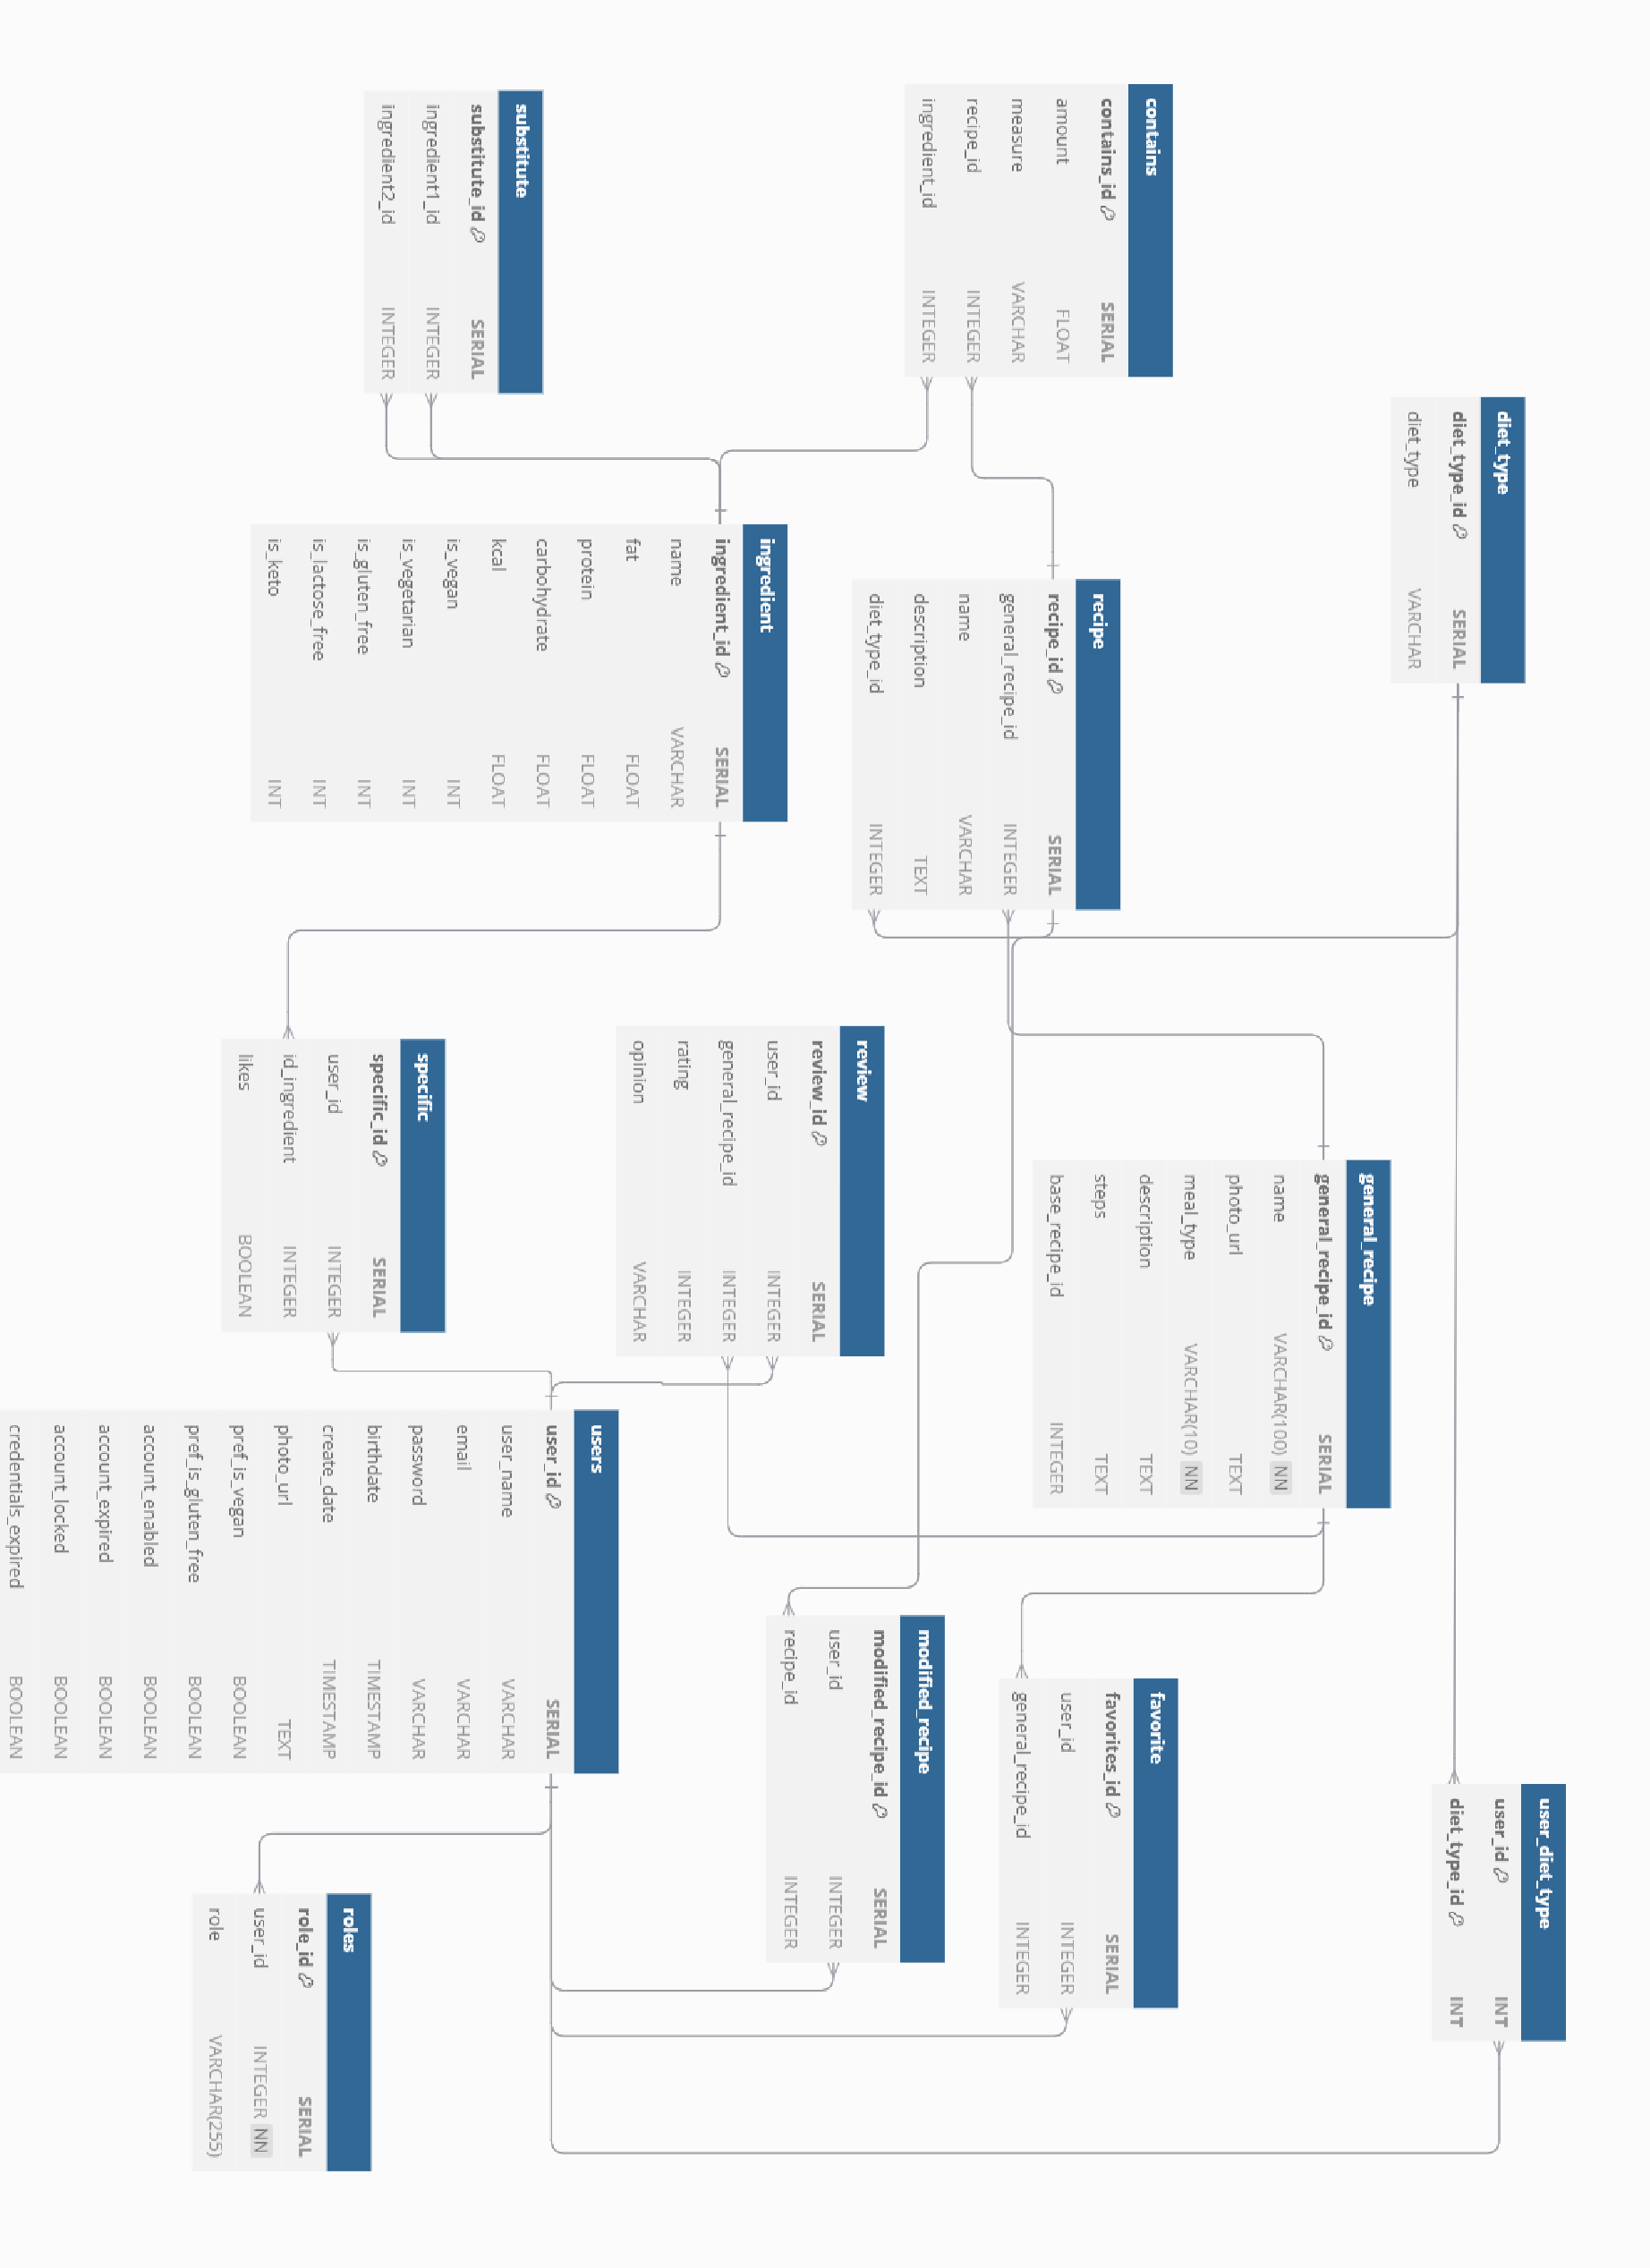
\includegraphics[width=\textwidth]{meta/pdf_attachments/schema_pdf.pdf}
    \caption{Database schema.}
    \label{fig:schema}
\end{figure}
The data dictionary is available at \textbf{Appendix B} \ref{chapter:appendixB}. 
\section{Transformations}
\chapterauthor{Kamil Dędza}
\par
API requests were executed using the Python requests library \cite{Requests}. To ensure security and prevent unauthorized access, the specific API keys and application IDs were stored in an environment file (.env), which was not exposed to the public or included in the source code of our repository. This approach ensures efficient and safe usage of API \cite{nutritionix}. 
{
\begin{minted}[linenos, frame=single]{python}
headers = {
            'Content-Type': os.getenv('CONTENT_TYPE'),
            'x-app-id': os.getenv('X_APP_ID'),
            'x-app-key': os.getenv('X_APP_KEY')
        }
body = {
    "query": ingredient # parameter with name of particular ingredient  
}
try:
    response = requests.post(
        'https://trackapi.nutritionix.com/v2/natural/nutrients',
        headers=headers,
        data=json.dumps(body)
    ).json()
except requests.exceptions.RequestException as e:
    print(f"Error while getting the data: {e}") 
\end{minted}
\captionof{figure}{Headers safely stored}
\label{fig:python-requests}
}

Moving forward, after having created the target tables and finding appropriate data sources, it is time to actually load the data. The responses come with data, which need to be transformed. Then and only then are we able to make use of these resources. We have organized our structure in such a way that for each table we have created a Python script, which transforms the data and generates files which later can be loaded into the database. Whole process follows a standard, production approach called ETL meaning extraction, transformation, and loading phases,which are used to migrate heterogeneous data from one or more data sources into a target system \cite{ETL-process}.
\par
To start with, the code snippet in Figure \ref{fig:python-requests} presents a simple extraction and transformation of the source fields into more of our desired structure.

\clearpage % Move the figure and everything after it to a new page

{
\begin{minted}[linenos, frame=single]{python}
name = response.get('strMeal')  # Validate 'strMeal' existence and value
if not name:
    return False
# Extract and clean fields
name = name.replace("'", "")
instructions = (response.get('strInstructions', "").replace("'", "")
                .replace("\n", " ").replace('\r', " "))
pho_url = response.get('strMealThumb', "").replace("'", "")
\end{minted}
\captionof{figure}{Extraction of fields from JSON response}
\label{fig:python-requests}
}
In majority of cases, this type of simple extraction is enough for our cases, meaning finding the proper field in response, then applying some cleaning function, in that case replace \cite{python-replace}, which ensures that the input is properly formatted. What is worth mentioning, it is also safe to use this approach from Figure \ref{fig:python-requests} even if there is no such field with a particular name, because then the second parameter from \texttt{get()}  function is returned, in our case it would be an empty string.
\par
For some tables it was necessary to get the primary key of other tables. One example of such usage can be the substitute table. The ingredient pairs are stored in the plain txt file as key and value pairs. So at first, we loaded the file, then we fetched the keys of ingredients from the pairs from an already existing table. If both were found, then we can save them into a file, and then load them into a table. So for this scenario, we have to keep in mind that the order of execution plays a role. Without an ingredient table we are not able to add the substitutes.
{
\begin{minted}[linenos, frame=single]{python}
with open(self.substitutes_map, mode='r', encoding='utf-8') as file:
    substitutes_map = csv.reader(file)
    for lines in substitutes_map:
        ingredient_1 = lines[0].lower().replace("'", "").replace(",", "")
        ingredient_2 = lines[1].lower().replace("'", "").replace(",", "")
        id_ingredient_1 = self.get_id("ingredient", "ingredient_id",
                                      ingredient_1.replace("'", ""))
        id_ingredient_2 = self.get_id("ingredient", "ingredient_id",
                                      ingredient_2.replace("'", ""))
        if id_ingredient_1 is None or id_ingredient_2 is None:
            print(f"Missing ID for {id_ingredient_1} or {id_ingredient_2}")
            return
        else:
            with open("substitutes_table.txt", "w", encoding='utf-8') as sub_file:
                # saving to file
                sub_file.write(f"DEFAULT,{id_ingredient_1},{id_ingredient_2}")
\end{minted}
\captionof{figure}{Fetching the primary keys of existing ingredients to make substitutes}
\label{fig:Mapping ingredients from external file}
}
The load phase, the final stage of the ETL process, involves transferring the cleaned and transformed data into the target data repository, which in this case is a Google Cloud Platform (GCP) PostgreSQL \cite{Postgres} instance. To maintain the security best practices, here we have again made use of the .env file, where we keep all our secret keys and password, without exposing them to public repositories. It also helps with future development of the code, making it easy to change for example password or user name. Our script takes the table name and path to a file which we want to load, and then after creating a query we execute it with the help of a \texttt{cursor} \cite{python-cursor}. Once created, this object allows developers to execute SQL statements like select, update, insert and delete. It also enables operations such as commit and rollback, making it easier to control changes. Query uses \texttt{\%s}  placeholders and passes data as a parameter to \texttt{cursor.execute()}. This ensures the database handles escaping and type conversion properly, avoiding SQL injection.
{
\begin{minted}[linenos, frame=single]{python}
PARAMS = {
    'dbname': os.getenv('GCP_DB_NAME'),
    'user': os.getenv('GCP_DB_USER'),
    'password': os.getenv('GCP_DB_PASSWORD'),
    'host': os.getenv('GCP_DB_HOST'),
    'port': os.getenv('GCP_DB_PORT')
}
def load_file_to_database(file_name, table_name):
    try:
        # connect to the PostgreSQL database and create a cursor
        connection = psycopg2.connect(**PARAMS)
        cursor = connection.cursor()
         # open the file and read lines
        with open(file_name, 'r', encoding='utf-8') as file:
            for line in file:
                row_data = tuple(line.strip().split(','))  # convert to tuple
                # construct the query with placeholders
                placeholders = ', '.join(['%s'] * len(row_data))
                query = f"INSERT INTO {table_name} VALUES ({placeholders});"
                try:
                    cursor.execute(query, row_data)  # pass row_data as parameters
                except (Exception, psycopg2.DatabaseError) as error:
                    print(f"Error while inserting row: {error}")
                    connection.rollback()  # roll back if there's an error
                else:
                    connection.commit()
\end{minted}
\captionof{figure}{Connection to GCP PostgreSQL instance and execution of the query}
\label{fig:Load to DB}
}
\par
All missing or empty values in the dataset were systematically identified and addressed. Intuitive dummy values, such as \texttt{n/a}(not available) for text fields were used to ensure clarity and maintain consistency in the data. To ensure that there are no anomalies in our database, we provided necessary checks and constraints. All columns that are referencing to another table, hence storing a foreign key were marked as such, so only the values existing in the table that they are pointing to are possible. For other columns, for example, \texttt{name} in the \texttt{general\_recipe} table is restricted by the \texttt{NOT NULL}  statement, which prevents adding ingredients without a name. Columns, where range of values is expected are also limited with proper check. Taking as an example the 'kcal' column from table 'ingredient', we know that it should only accept values from range 0 to 900.
{
\begin{minted}[linenos, frame=single]{sql}
alter table ingredient
alter column name set not null;
alter table ingredient
add constraint expected_macro check (fat >= 0  and carbohydrate >= 0 
and protein >= 0 and kcal >= 0
and fat <= 100 and carbohydrate <= 100 and protein <= 100
and kcal <= 900);
alter table  ingredient
add constraint valid_flags check (is_keto in (0,1) and is_vegan in (0,1)
and is_gluten_free in (0,1) and
is_vegetarian in (0,1) and is_lactose_free in (0,1));
\end{minted}
\captionof{figure}{Constraints on ingredient table}
\label{fig:Contraints}
}
\par
To sum up, our data handling process starts with making use of existing and open APIs. Then we suit the data for our purposes, which includes cleansing and transformation. When all the information is ready to be stored in persistent storage, we load them into the PostgreSQL \cite{Postgres} service for databases provided by GCP. After that step, our other services can take advantage of such data, and empower our solution with valuable features and information.

